\documentclass[sigconf]{webmedia}

\AtBeginDocument{
  \providecommand\BibTeX{{
    \normalfont B\kern-0.5em{\scshape i\kern-0.25em b}\kern-0.8em\TeX}}}

\settopmatter{printacmref=false, printfolios=false}

\proceedingsDetails [WTVDI'2026]{IX Workshop Futuro da TV Digital Interativa (WTVDI 2026). Anais Estendidos do XXXII Simpósio Brasileiro de Sistemas Multimídia e Web}{2026}{Lavras/MG, Brazil}
\ISSN{2596-1683}

\usepackage{tikz}
\usetikzlibrary{positioning,shapes,arrows,matrix,shapes.geometric,fit,backgrounds,calc}
\usepackage{subcaption}
\usepackage{listings}
\usepackage{stfloats}
\usepackage{booktabs}
\usepackage{fontawesome5}

\lstset{
  basicstyle=\ttfamily\small,
  columns=fullflexible,
  keepspaces=true,
  breaklines=true,
  frame=single,
  showstringspaces=false
}

\begin{document}

\title{A new Ginga Developer Ecosystem with \texttt{ginga.org.br} portal, and \texttt{ginga-playground} and \texttt{ginga-code} tools}

\author{Alan L. V. Guedes}
\email{a.guedes@reading.ac.uk}
\affiliation{%
  \institution{University of Reading}
  \country{UK}
}

\author{Paulo Victor Borges}
\orcid{0009-0002-3620-477X}
\email{paulo.victor.lima15@gmail.com}
\affiliation{%
  \institution{PUC-Rio}
  \country{Brazil}
}

\author{Daniel Moraes}
\orcid{0000-0003-2995-3115}
\email{danielmoraes@telemidia.puc-rio.br}
\affiliation{%
  \institution{PUC-Rio}
  \country{Brazil}
}

\author{Sergio Colcher}
\orcid{0000-0002-3476-8718}
\email{colcher@puc-rio.br}
\affiliation{%
  \institution{PUC-Rio}
  \country{Brazil}
}

\renewcommand{\shortauthors}{Guedes et al.}

\begin{abstract}
The authoring and execution of Ginga-NCL/HTML5 applications for digital television (DTV) have long been constrained by the lack of developer accessibility to lightweight prototyping and testing tools. In this paper, we present a new \textbf{Ginga Developer Ecosystem} designed to lower the barrier to entry for Ginga development. The ecosystem integrates three pillars: (1) \texttt{ginga.org.br}, a web portal using a modern static website generator to host fully reviewed Ginga documentation and the NCL Handbook; (2) \texttt{ginga-playground}, a browser-native code editor and execution of Ginga-NCL/HTML5 applications; and (3) \texttt{ginga-code}, a Visual Studio Code extension acting as a launch tool of Ginga-NCL/HTML5 applications directly from the IDE.
\end{abstract}

\keywords{Ginga-NCL, Developer Ecosystem, Web Workbench, VS Code Extension, Debug Bridge, CanvasKit, Headless Execution}


\begin{teaserfigure}
\centering
\begin{subfigure}[b]{0.48\textwidth}
  \centering
  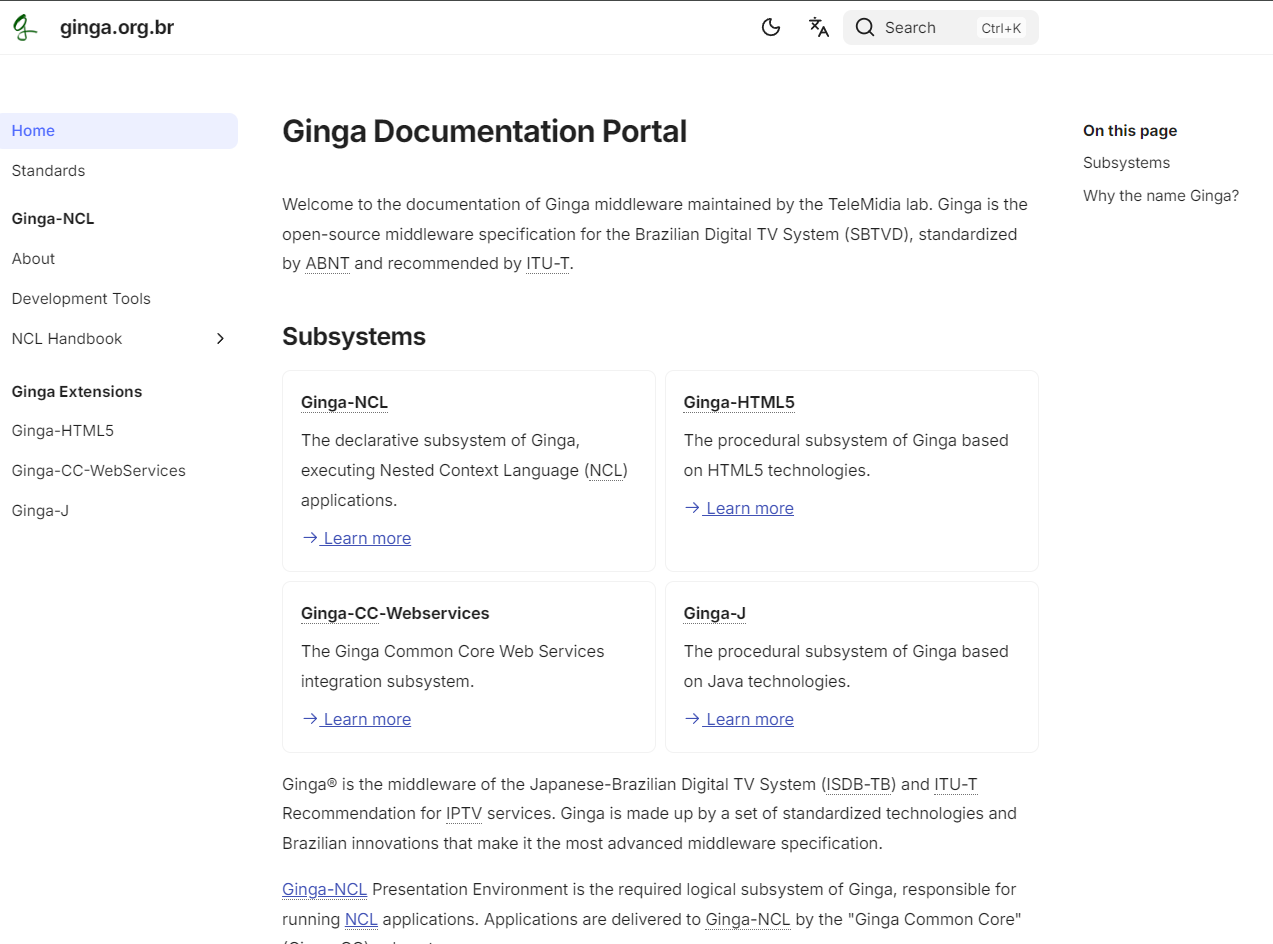
\includegraphics[width=\textwidth]{assets/portal1.png}
  \caption{Portal Landing Page}
  \label{fig:portal1}
\end{subfigure}
\hfill
\begin{subfigure}[b]{0.48\textwidth}
  \centering
  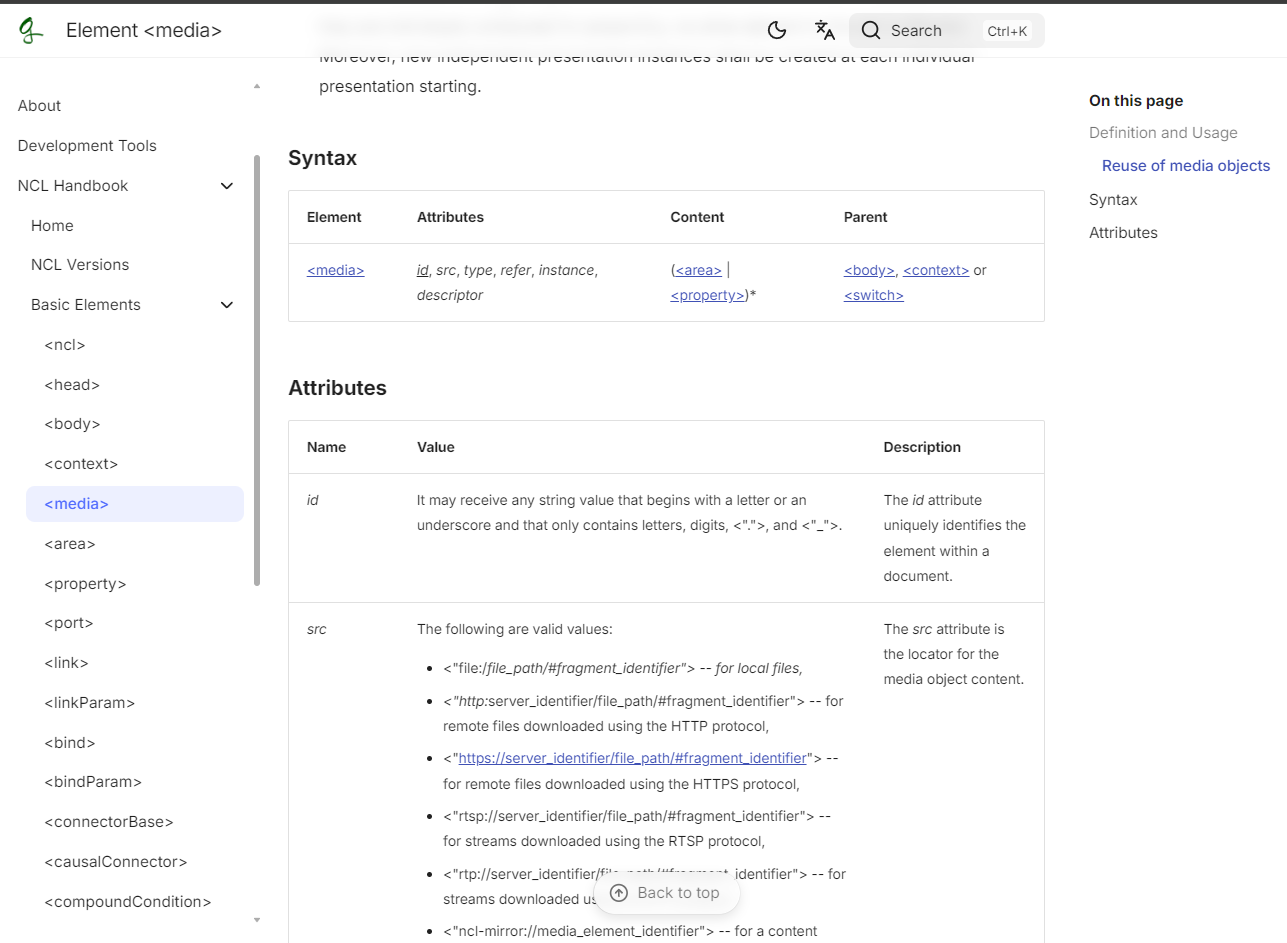
\includegraphics[width=\textwidth]{assets/portal2.png}
  \caption{Portal Documentation}
  \label{fig:portal2}
\end{subfigure} \\[2ex]
\begin{subfigure}[b]{0.48\textwidth}
  \centering
  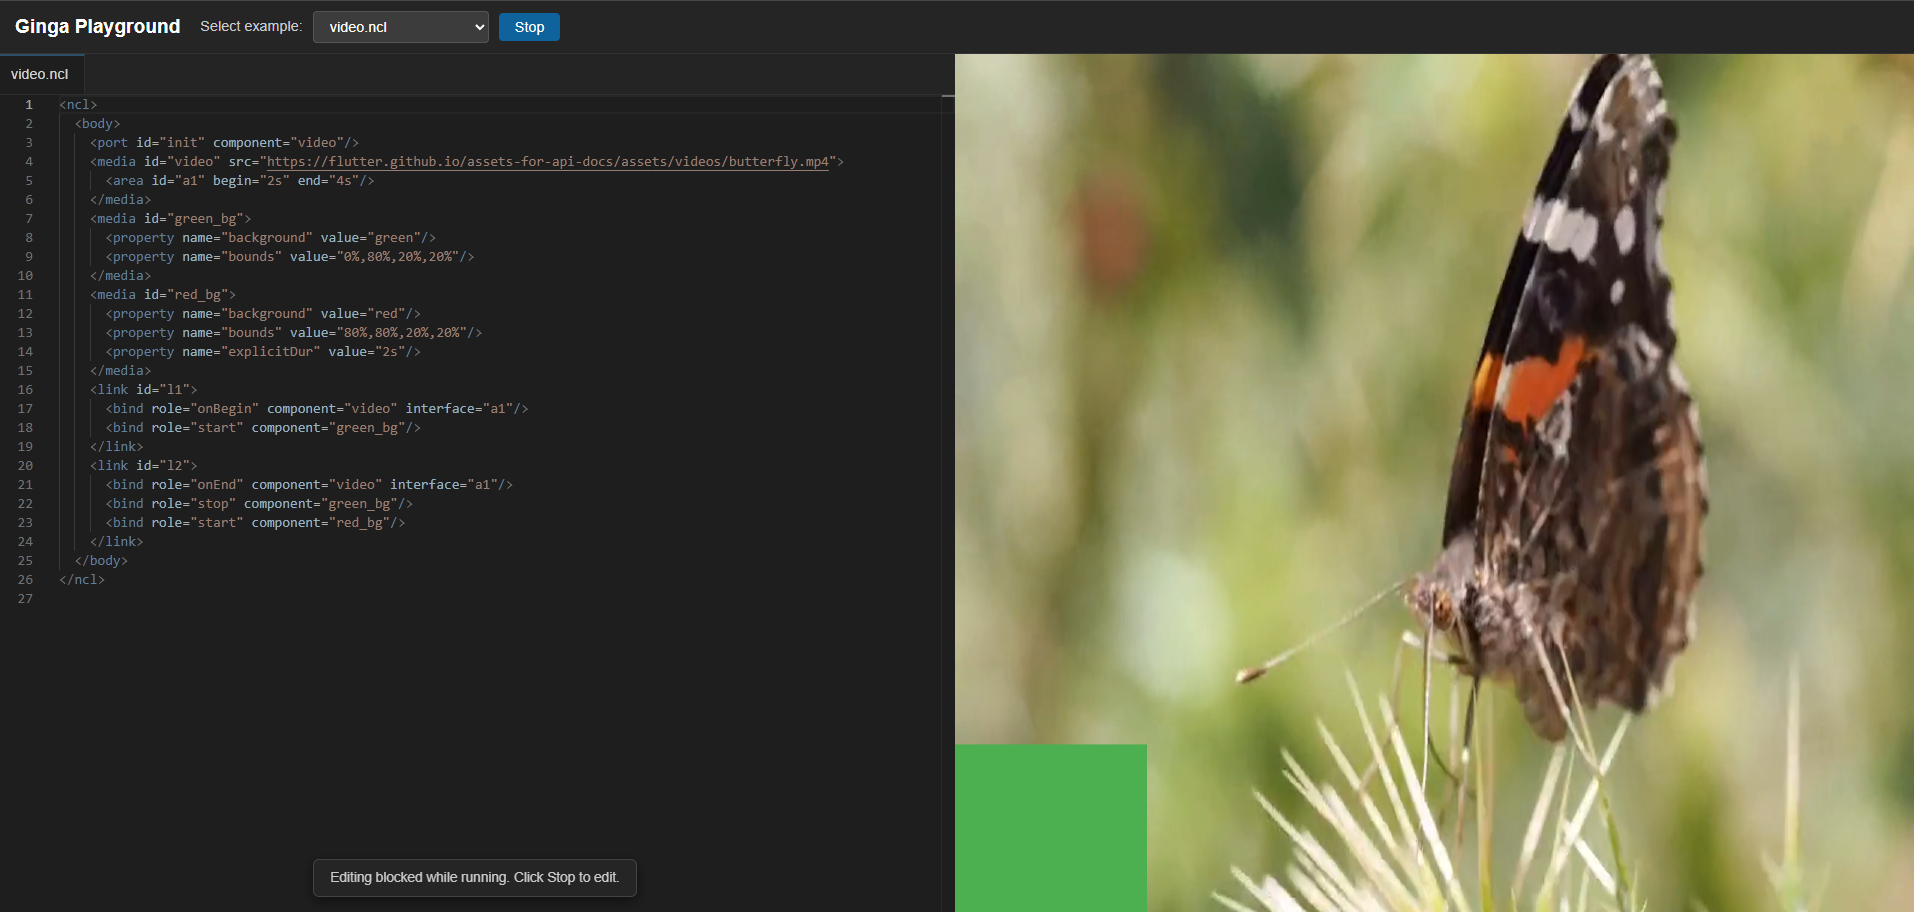
\includegraphics[width=\textwidth]{assets/playground.png}
  \caption{Ginga Playground at Web}
  \label{fig:playground}
\end{subfigure}
\hfill
\begin{subfigure}[b]{0.48\textwidth}
  \centering
  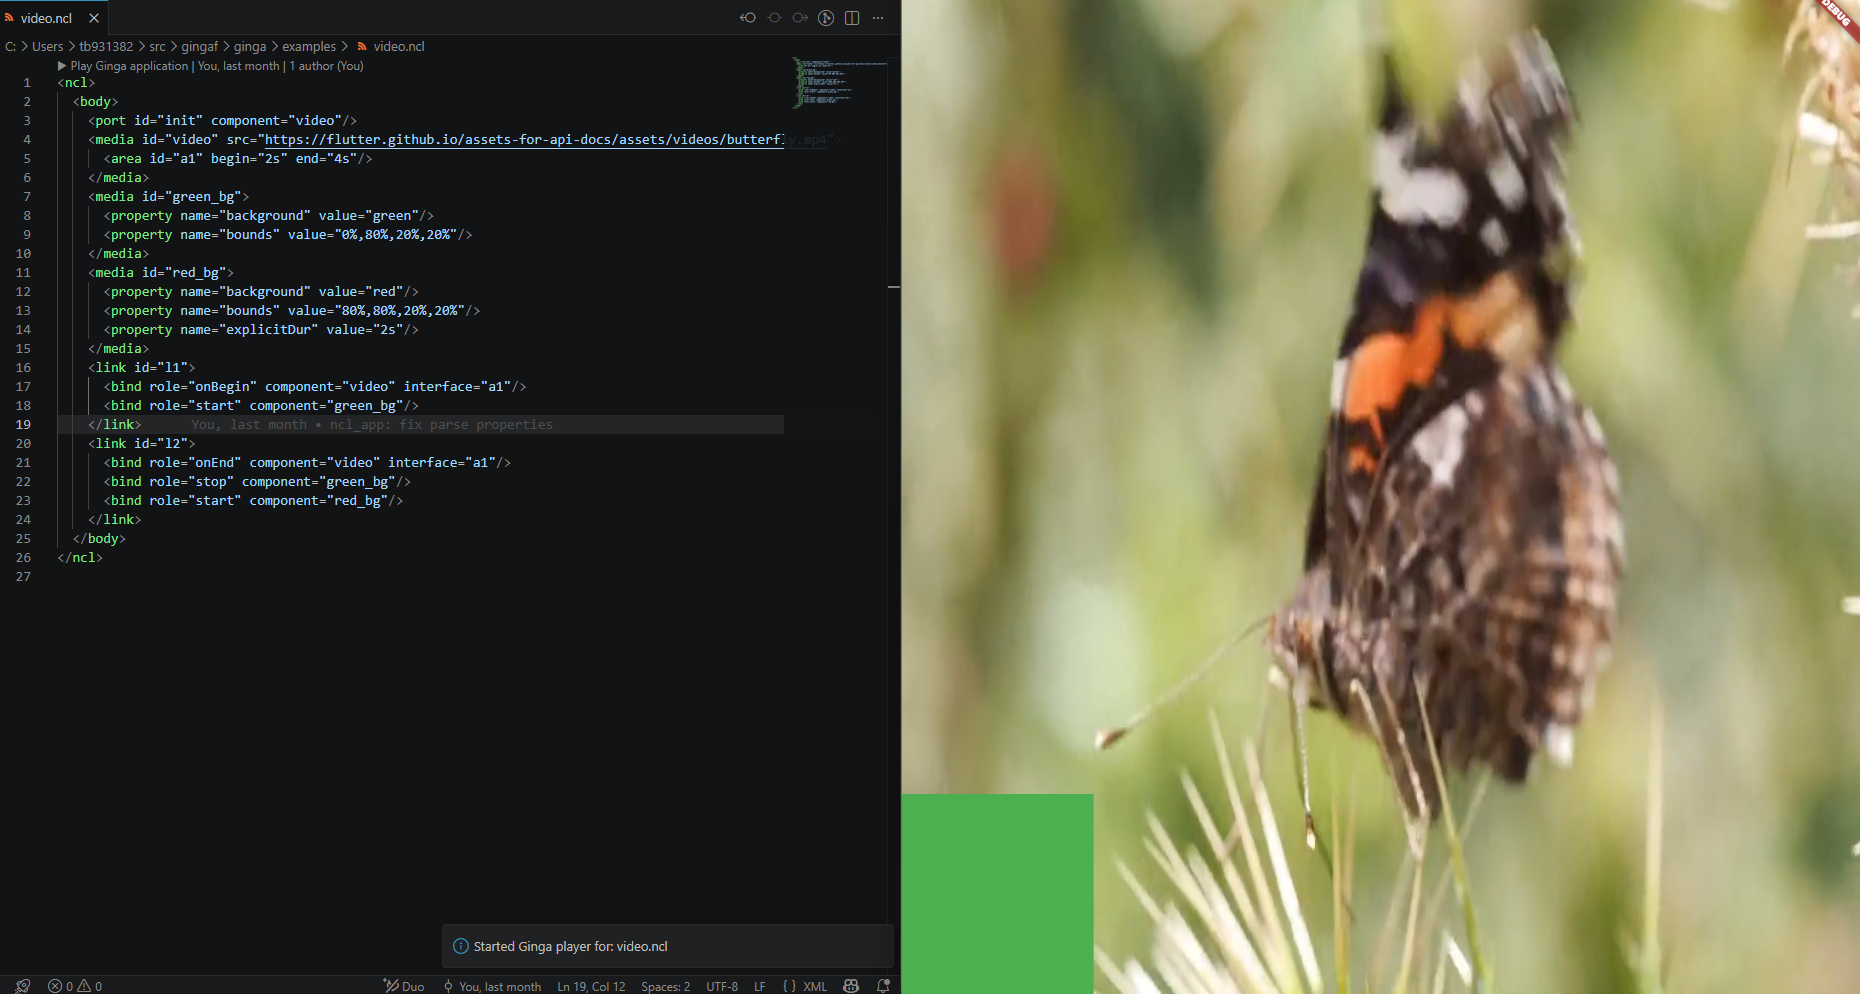
\includegraphics[width=\textwidth]{assets/vscode.png}
  \caption{Ginga VS Code Extension at Desktop}
  \label{fig:vscode}
\end{subfigure}
\Description{Screenshots of the Ginga Developer Ecosystem components: the main portal landing page, interactive API documentation, web-based playground workbench, and the VS Code debugger extension.}
\caption{Ginga Developer Ecosystem interfaces: portal landing page (a), documentation (b), playground workbench (c), and VS Code extension (d).}
\label{fig:ecosystem_landing_hero}
\end{teaserfigure}
\maketitle

\section{Introduction}
\label{sec:intro}

The Ginga middleware is the international standard for interactive digital television by both the ITU-T~\cite{ITU_H761} and the Brazilian Digital Terrestrial Television System (SBTVD)~\cite{abnt_15606_2_2023}. Ginga utilizes the Nested Context Language (NCL)---an XML-based declarative multimedia language. As the official presentation engine for interactive television applications, the Ginga standard is legally mandated and installed on 100\% of certified Digital TV sets and set-top boxes sold in Brazil and several other Latin American countries adopting the ISDB-T framework.

Despite its standardization and wide adoption across SBTVD and international broadcast networks, the lack of developer accessibility to testing and prototyping tools has historically been the primary barrier for Ginga developers. Traditional developer workflows require configuring native middleware libraries, installing platform-specific dependencies, or relying on heavy set-top box (STB) hardware emulators~\cite{lima2018ginga, moreno2010conciliando}. To overcome this lack of accessibility, we introduce a new \textbf{Ginga Developer Ecosystem}, an open-source development suite unifying web authoring, portal demonstration, and IDE launching. Built around the modular \texttt{gingaf} presentation engine~\cite{gingaf2026}\footnote{\url{https://github.com/ginga-org-br/gingaf}}, the ecosystem integrates three core pillars: the \texttt{ginga.org.br} portal\footnote{\url{https://ginga-org-br.github.io/ginga.org.br/}}, \texttt{ginga-playground}\footnote{\url{https://ginga-org-br.github.io/gingaf/playground/}}, and \texttt{ginga-code}\footnote{\url{https://marketplace.visualstudio.com/items?itemName=ginga-org-br.ginga-code}}.

The remainder of this paper is structured as follows. Section~\ref{sec:related} reviews related work in Ginga middleware tooling. Section~\ref{sec:ecosystem} details the architecture of the Ginga Developer Ecosystem and its core pillars. Finally, Section~\ref{sec:remarks} outlines final remarks and future directions.

\section{Related Work}
\label{sec:related}

The development of Ginga players has historically been led by the TeleMídia Lab at PUC-Rio, producing several versions. PUC-Rio Ginga v0.13.6~\cite{ginga2013,moreno2010conciliando}\footnote{\url{https://github.com/TeleMidia/ginga/releases/tag/v0.13.6}} was designed for resource-constrained early-generation digital TV receivers. PUC-Rio Ginga v1.0~\cite{ginga2018,dodsworth2018dynamic} modernised the renderer and moved to a mono-threaded model inspired by synchronous execution. However, such implementations share a fundamental limitation: they are deeply tethered to native desktop libraries, making web execution impossible. Another earlier work was WebNCL~\cite{webncl2013}, which provided a web-based NCL presentation engine but did not support Lua scripting.

The closest related works to our initiative are NuGinga~\cite{nuginga18} and NuGinga Playcode~\cite{nuginga_playcode20}. Developed by Sidia, NuGinga~\cite{nuginga18} introduced a Node.js-based Ginga middleware engine. Subsequently, NuGinga Playcode~\cite{nuginga_playcode20} introduced a Node.js-based authoring tool for Ginga-NCL and NCLua using cross-compilation techniques; however, given its Node.js-based architecture, it requires server-side execution infrastructure. Also, it lacks support for Ginga-HTML5 application coding. In contrast, the proposed Ginga Developer Ecosystem and its \texttt{ginga-playground} workbench provide a fully client-side, zero-installation environment that natively supports both Ginga-NCL and Ginga-HTML5 (via CCWS integration).

\section{Ginga Developer Ecosystem} \label{sec:ecosystem}

\begin{figure}[h]
\centering
\begin{tikzpicture}[
  node distance=1.2cm and 1.5cm,
  block/.style={draw=black!70, fill=black!5, rectangle, rounded corners=4pt, minimum width=3.2cm, minimum height=1.0cm, align=center, font=\small\sffamily},
  dev/.style={draw=black!70, fill=black!5, circle, minimum size=1.5cm, align=center, font=\scriptsize\sffamily},
  arrow/.style={draw, ->, >=stealth, line width=1pt}
]

\node [block] (gingaf) at (0,2) {\href{https://github.com/ginga-org-br/gingaf}{\textbf{\texttt{gingaf} Engine}}};
\node [block] (vscode) at (-2.2,0) {\href{https://marketplace.visualstudio.com/items?itemName=ginga-org-br.ginga-code}{\textbf{\texttt{ginga-code}}}};
\node [block] (playground) at (2.2,0) {\href{https://ginga-org-br.github.io/gingaf/playground/}{\textbf{\texttt{ginga-playground}}}};
\node [block] (portal) at (0,-2) {\href{https://ginga-org-br.github.io/ginga.org.br/}{\textbf{\texttt{ginga.org.br} Portal}}};
\node [dev] (dev1) at (-2.2,-4.2) {{\Large\faUser}\\[0.1ex] Developer at\\[-0.5ex] Desktop};
\node [dev] (dev2) at (2.2,-4.2) {{\Large\faUser}\\[0.1ex] Developer at\\[-0.5ex] Browser};

\draw [arrow] (vscode.north) -- (gingaf.south west);
\draw [arrow] (playground.north) -- (gingaf.south east);
\draw [arrow, dashed] (portal.north -| vscode.south east) -- node[left, font=\scriptsize] {Suggests} (vscode.south east);
\draw [arrow, dashed] (portal.north -| playground.south west) -- node[right, font=\scriptsize] {Links to} (playground.south west);
\draw [arrow, dashed] (dev1) -- node[below, font=\tiny, pos=0.4] {Reads docs} (portal);
\draw [arrow, dashed] (dev2) -- node[below, font=\tiny, pos=0.4] {Reads docs} (portal);
\draw [arrow] (dev1.north) -- node[left, font=\scriptsize] {Runs application} (vscode.south);
\draw [arrow] (dev2.north) -- node[right, font=\scriptsize] {Runs application} (playground.south);

\end{tikzpicture}
\caption{Components of the new Ginga Developer Ecosystem.}
\label{fig:component_diagram}
\end{figure}

The proposed new Ginga Developer Ecosystem consists of components built on top of the \texttt{gingaf} presentation engine~\cite{gingaf2026}. The ecosystem isolates the core Ginga execution logic, allowing it to run cross-platform and target web sandboxes and desktop IDEs. As illustrated in Figure~\ref{fig:component_diagram}, the ecosystem accommodates different developer profiles:
\begin{itemize}
  \item The \texttt{Developer at Desktop} profile represents advanced users or academics developing new Ginga extensions.
  \item The \texttt{Developer at Browser} profile represents new users learning Ginga-NCL development in a lightweight sandbox.
\end{itemize}

These components are organized into the following sections.

\subsection{\texttt{gingaf}}

The \texttt{gingaf} presentation engine is an open-source, cross-platform Ginga digital television middleware player built on Dart and the Flutter framework. Unlike traditional native middleware architectures that tightly bind execution state machines directly to OS graphics contexts (such as SDL or GTK) and native AV pipelines, \texttt{gingaf} introduces a decoupled layered architecture that strictly separates headless document logic components from visual UI components.

The core execution engine (\texttt{ncldoc} / \texttt{NCLDocument}) manages the declarative NCL state machine, temporal synchronization loops, and reactive DOM events entirely in pure and cross-platform Dart code. The ginga presentation layer sits above this logic core, leveraging Flutter to paint visual elements natively on desktop and mobile targets or onto a hardware-accelerated CanvasKit surface (a WebAssembly build of Skia) for in-browser web execution. The engine natively supports \texttt{Ginga-NCL} (including embedded Lua scripting via a pure Dart interpreter), \texttt{Ginga-HTML5}, and \texttt{Ginga-CC-Webservices} (CCWS REST APIs exposed via an internal HTTP server). This modular design powers the rendering surfaces of the web workbench (\texttt{ginga-playground}) and desktop execution targets (\texttt{ginga-code}).

\subsection{New \texttt{ginga.org.br} Portal}

The official portal \texttt{ginga.org.br}\footnote{\url{https://ginga-org-br.github.io/ginga.org.br/}} serves as the central hub of the Ginga Developer Ecosystem. This new version converts the old portal architecture, featuring fully reviewed text and documentation with multilingual support across three languages: Portuguese, Spanish, and English. It is built using Zensical\footnote{\url{https://zensical.org/}}, a modern static website generator. The portal integrates specification documentation and already includes the complete NCL Handbook (Figure~\ref{fig:portal2}) alongside live code examples.

\subsection{\texttt{ginga-playground}}

The \texttt{ginga-playground} is a browser-native code workbench that provides an interactive execution environment running entirely on the client side without native plugins. It combines a code editor built on Monaco Editor~\cite{monaco_editor} and a web deployment of the \texttt{gingaf} presentation engine. To ensure document persistence across sessions, the workbench leverages HTML LocalStorage\footnote{\url{https://html.spec.whatwg.org/multipage/webstorage.html}} to store user files and enable seamless editing. Furthermore, the playground comes pre-loaded with a catalog of example NCL applications, enabling developers to instantly explore, edit, and preview interactive multimedia scenarios.

\subsection{\texttt{ginga-code}}

For desktop development, the \texttt{ginga-code}\footnote{\url{https://marketplace.visualstudio.com/items?itemName=ginga-org-br.ginga-code}} extension enables execution of Ginga-NCL and HTML5 applications directly within Visual Studio Code. The extension automatically downloads the native \texttt{gingaf} desktop binary matching the host operating system to serve as an IDE launcher. It then provides an interactive button within the IDE interface that allows developers to launch and execute the Ginga application currently open in the active editor. 

\section{Final Remarks}
\label{sec:remarks}

The Ginga Developer Ecosystem bridges web distribution and tool launcher interfaces for NCL digital television applications. By integrating \texttt{ginga.org.br}, \texttt{ginga-playground}, and \texttt{ginga-code} on top of the \texttt{gingaf} engines, the suite eliminates environment setup friction and provides instant preview capabilities. 

Future work will focus on expanding comprehensive \texttt{ginga.org.br} documentation for \texttt{Ginga-HTML5} and \texttt{Ginga-CCWS}, as well as introducing an NCL Language Server Protocol (LSP) provider for static semantic verification.

\bibliographystyle{ACM-Reference-Format}
\bibliography{references}

\end{document}
